\documentclass[11pt,twocolumn]{article}
\usepackage{lmodern,setspace,amsmath,amssymb,amsfonts,amsthm,graphicx,multicol,grffile,float,csvsimple}
\usepackage[a4paper, top=0.9in, bottom=1.05in, left=1.05in, right=1.05in]{geometry}
\usepackage[polish]{babel}
\usepackage[utf8]{inputenc}
\usepackage[T1]{fontenc}
\title{Algorytmy i struktury danych - Algorytmy grafowe}
\author{Dariusz Max Adamski}
\date{}

\begin{document}

\maketitle



\section*{Wstęp}

W tym sprawozdaniu porównywana będzie efektywność różnych reprezentacji grafów, 
przez mierzenie średniego czasu sprawdzania istnienia krawędzi. 
Oceniona będzie także implementacja sortowania topologicznego, 
używająca listy incydencji do reprezentacji danych.


\section*{Metodologia}

Pomiary wykonywane były na grafach o ilości wierzchołków $|V|$ od $100$ wierzchołków do $1500$ wierzchołków, z krokiem $100$ (15 punktów pomiarowych).

Przed mierzewiem czasu sprawdzania krawędzi, wczytywany jest z pliku tekstowego, 
losowo wygenerowany nieskierowany graf, o ilości wierzchołków $|V|$ 
i nasyceniu krawędziami 0.6, do macierzy sąsiedztwa ,,AM''.

Następnie dane są kopiowane do macierzy incydencji ,,IM'', listy krawędzi ,,EL'' oraz listy incydencji ,,AL''.

Tworzona jest także tablica $S$ o wielkości $|V|$ z warościami od 0 do $|V|-1$. 
Po utworzeniu tablica jest losowo tasowana, tak aby wartość $S_i$ nie była równa $i$.

Podczas mierzenia czasu, dla każdego indeksu $i$ od 0 do $|V|-1$ sprawdzana 
jest obecność krawędzi od wierzchołka $i$ do wierzchołka $S_i$. 
Na końcu zmierzony czas jest dzielony przez $|V|$.

Aby zmierzyć czas sortowania topologicznego, wczytywany jest z pliku tekstowego 
losowo wygenerowany skierowany graf bez cykli ,,DAG'', o ilości wierzchołków $|V|$ 
i nasyceniu krawędziami 0.3, bezpośrednio do macierzy listy incydencji ,,AL''. 
Następnie mierzony jest czas sortowania.

Optymalizacje kompilatora zostały wyłączone flagą ,,-O0''. 
Czas wykonywania był mierzony w nanosekundach.


\section{Istnienie krawędzi}

\begin{figure}[h]
	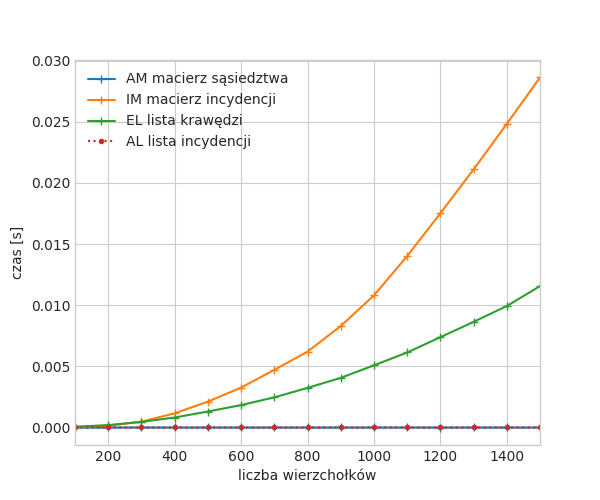
\includegraphics[width=\linewidth]{wyszukaj.png}
	\caption{Średni czas sprawdzania istnienia krawędzi \label{wyszukaj}}
\end{figure}

\begin{figure}[h!]
	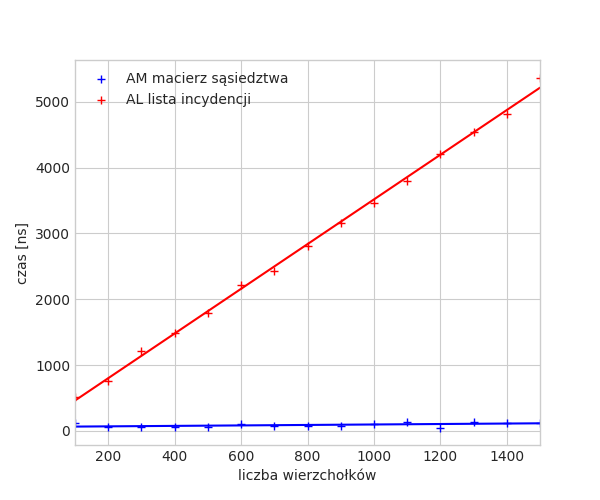
\includegraphics[width=\linewidth]{wyszukaj-nano.png}
	\caption{Średni czas sprawdzania istnienia krawędzi (ns) \label{wyszukaj-nano}}
\end{figure}

Czas sprawdzania istnienia krawędzi dla AM ma złożoność $O(1)$. 
Dla AL złożoność tej operacji to $O(|V|)$. 
Natomiast używając IM lub EL ta czynność ma złożoność $O(|E|)$.

W wygenerowanych grafach liczba wierzchołków to $|E|=\lfloor \phi (|V|^2+|V|) \rfloor$, 
gdzie $\phi$ jest współczynnikiem nasycenia krawędziami.
Dlatego właśnie dla IM i EL w tym przypadku $O(|E|) = O(|V|^2)$.

%Sprawdzenie czy krawędź istnieje w IM jest wolniejsze niż w EL ponieważ
%musimy wykonać dwa dodatkowe sprawdzenia wartości w tablicy, po jednym dla wierzchołka,
%podczas gdy w liście krawędzi j

Ponieważ $|V| \ll |E|$, w szczególnośći przy $\phi = 0.6$, 
wyniki dla AM i AL zostały przedstawione także na rysunku 2 (w nanosekundach).

\section{Sortowanie topologiczne}

\begin{figure}[h!]
	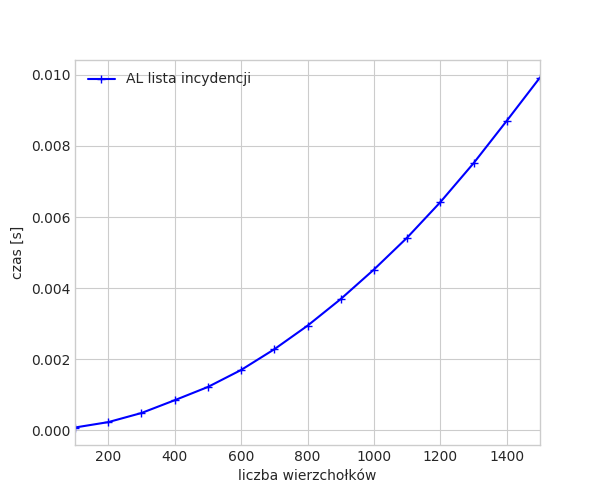
\includegraphics[width=\linewidth]{sortuj.png}
	\caption{Czas sortowania topologicznego \label{sortuj}}
\end{figure}

Czynność sortowania topologicznego ma złożoność $O(|V|+|E|)$.

Do reprezentacji grafu w sortowaniu topologicznym została wybrana lista incydencji AL. 

Głównym powodem była prostota implementacji. 
Podczas sortowania musimy odwiedzać sąsiadujące wierzchołki.
W AL mamy natychmiastowy dostęp do \emph{listy} sąsiadów znanego wierzchołka w czasie $O(1)$, 
co sprawia, że nie musimy konstruować listy następnych wierzchołków do odwiedzenia.

Pozostałe zalety i wady AL są opisane w następnej sekcji.

\section {Wnioski}

Ilość wymaganej pamięci przez AL nie jest duża, bo (tutaj) rzędu 
$O_p(|V|+|E|) = O_p(|V|^2)$. 
Dla rzadkiego grafu AL może zajmować nawet mniej pamięci niż AM.
W rzeczywistości im większe $\phi$ tym więcej pamięci jest wymagane, 
ale w przypadku sortowania topologicznego, przy $\phi = 0.3$, nie stanowi to dużego problemu.

Dobrą alternatywą jest AM która wymaga pamięci $O_p(|V|^2)$, 
ale w odróżnieniu od AL nie rośnie wraz z $|E|$ lub $\phi$. 
Znajdywanie sąsiadów za to zajmuje więcej czasu niż w AL, ma ono złożoność $O(|V|)$.
Inną wadą jest potrzeba kopiowania macierzy przy dodawaniu wierzchołków do grafu.

EL potrzebuje $O_p(|E|)$ pamięci, 
co daje w tym aspekcie przewagę nad AL oraz IM, ale nie nad AM.
Jednak znajdywanie sąsiadów jest czasochłonne bo ma złożoność $O(|E|)$.

IM wymaga $O_p(|V|\cdot|E|)$ pamięci co jest bardzo nieefektywne.
W dodatku operacje na tej reprezentacja są niewygodne oraz czasochłonne.
Wydaje się, że IM jest kumulacją najgorszych cech EL i AM.

Podsumowując, dla zadanych problemów, 
najlepszymi reprezentacjami grafu są lista incydencji AL, oraz macierz sąsiedztwa AM. 
Natomiast lista krawędzi EL i macierz incydencji IM okazały się nieefektywne.


\end{document}

